% Four pages for a non-technical reader: the stream in one picture, what the technology is, what it achieved in
% two days, and how to run the demo from GitHub. Build: latexmk -pdf voice_demo.tex
\documentclass[aspectratio=169,10pt]{beamer}
\usetheme{default}
\usecolortheme{seagull}
\setbeamertemplate{navigation symbols}{}
\setbeamertemplate{footline}{\hspace*{1.2em}\tiny Phasefield \textperiodcentered\ Marcel Crasmaru \textperiodcentered\ 22 November 2026 \textperiodcentered\ github.com/crasmarum/CNet \hfill \insertframenumber/\inserttotalframenumber\hspace*{1.2em}\vspace*{0.5em}}
\setbeamertemplate{itemize items}[circle]
\setbeamerfont{frametitle}{size=\large,series=\bfseries}
\setbeamercolor{frametitle}{fg=black!85}
\setbeamercolor{block title}{bg=black!8,fg=black!85}
\setbeamercolor{block body}{bg=black!3}
\setbeamersize{text margin left=1.2em,text margin right=1.2em}
\usepackage{booktabs}
\usepackage{xcolor}
\definecolor{accent}{RGB}{0,90,140}
\newcommand{\num}[1]{\textcolor{accent}{\textbf{#1}}}

\begin{document}

% ------------------------------------------------------------------ page 1: the picture
\begin{frame}[plain]
\vspace*{2mm}
\centering
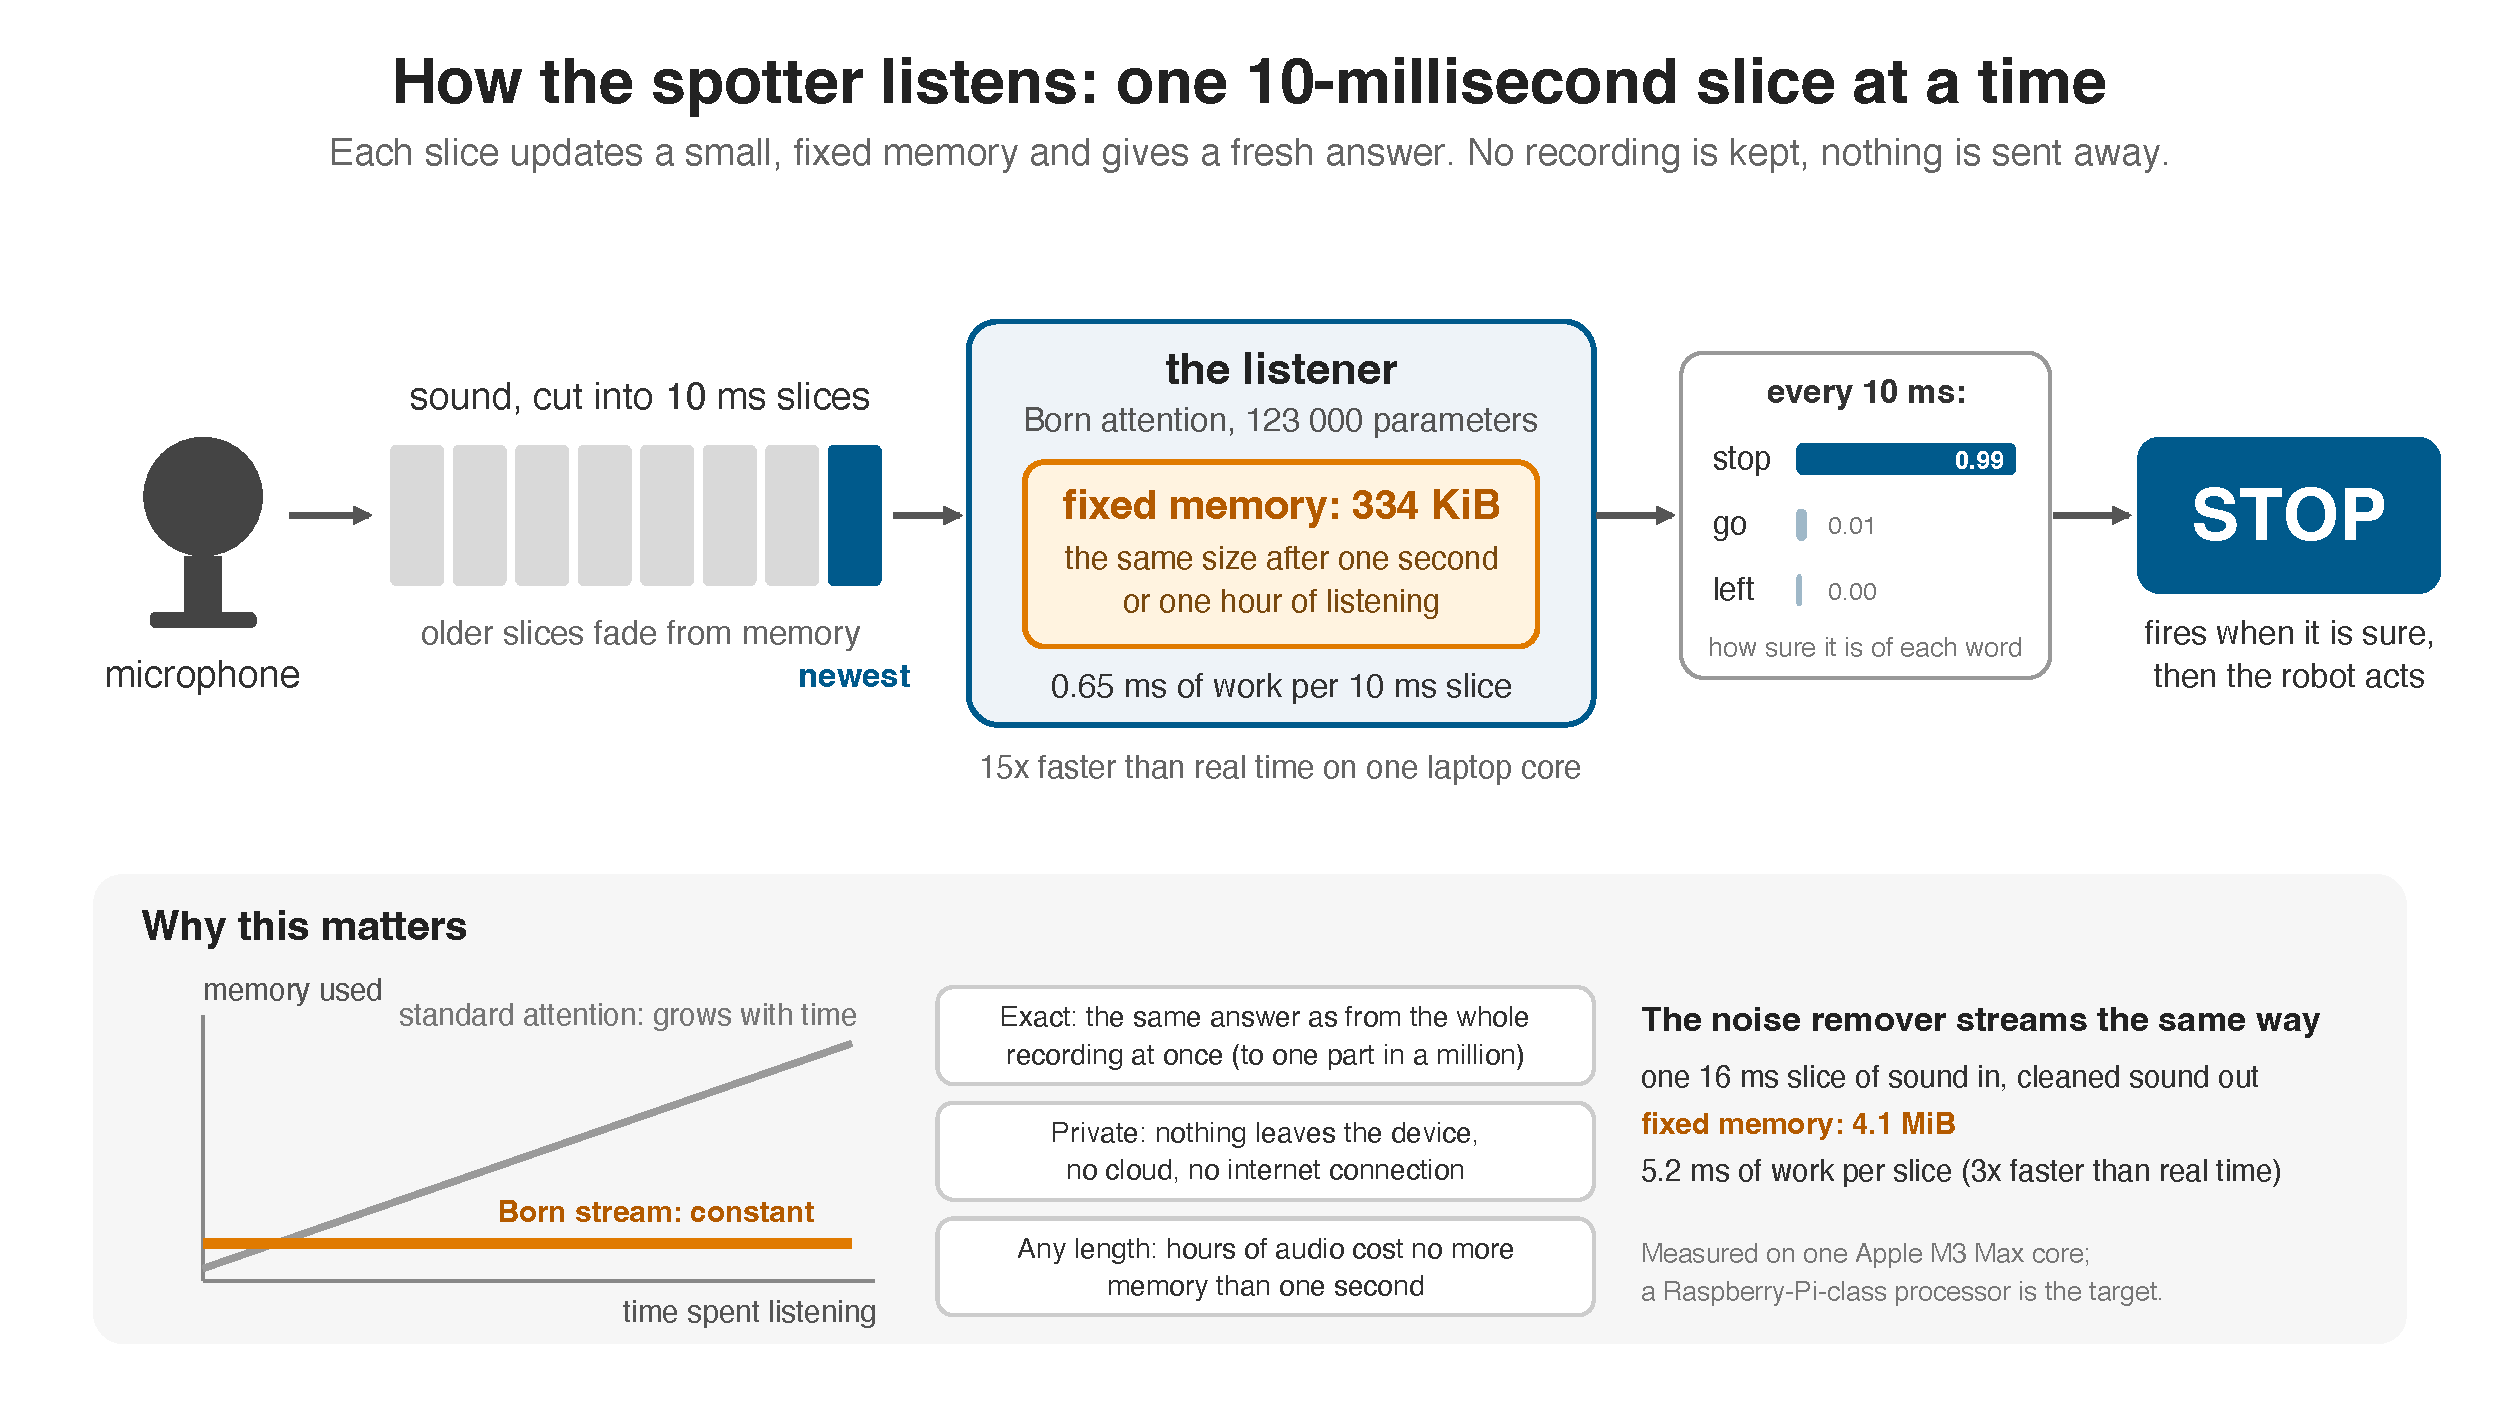
\includegraphics[width=0.95\paperwidth]{streaming_overview.pdf}
\end{frame}

% ------------------------------------------------------------------ page 2
\begin{frame}{Voice AI that listens all the time, on a tiny processor}
\small
\begin{columns}[T]
\begin{column}{0.54\textwidth}
\textbf{The problem.} Small robots, wearables and appliances must hear you continuously, with no cloud link, no graphics chip and a small battery. Today's speech models are built for short clips: they re-read the last second at every step, or they stream over a fixed window that forgets abruptly.

\medskip
\textbf{What we built.} \emph{Born attention} weighs earlier sound by a probability, as a measurement does in quantum physics. Its kernel has an exact recurrence (softmax attention has none), so the model runs \num{one 10-millisecond frame at a time}, with a memory that \num{never grows}, and the stream gives \num{exactly} the result the same model gives from the whole recording.

\medskip
\textbf{Two models, one stack.} A command spotter and a noise remover, trained from the raw waveform in our own framework (CNet: C++/CUDA, complex numbers built in) and run as streams on a plain CPU.
\end{column}
\begin{column}{0.44\textwidth}
\begin{block}{What the stream costs, one Apple M3 Max core}
\scriptsize\setlength{\tabcolsep}{3pt}
\begin{tabular}{@{}lrr@{}}
\toprule
 & Spotter & Denoiser \\
\midrule
memory between frames & 334 KiB & 4.1 MiB \\
compute per frame of audio & 0.65 / 10 ms & 5.2 / 16 ms \\
faster than real time & 15$\times$ & 3$\times$ \\
match with the offline model & 1 in 10$^6$ & 1 in 10$^5$ \\
model file & 1.4 MB & 6.8 MB \\
\bottomrule
\end{tabular}
\end{block}
\begin{block}{Against the alternatives}
\scriptsize
\begin{itemize}
\item \emph{Standard transformers}: memory grows with time, or a fixed window forgets abruptly.
\item \emph{Other linear-attention kernels}: also constant memory; the Born kernel was ahead of a gated-linear one at every matched checkpoint on spotting, 48 of 50 on denoising.
\item \emph{No attention}: 15 points of accuracy lost.
\end{itemize}
\end{block}
\end{column}
\end{columns}
\end{frame}

% ------------------------------------------------------------------ page 3
\begin{frame}{Two models in two days (20--22 November 2026)}
\small
\begin{columns}[T]
\begin{column}{0.52\textwidth}
\begin{block}{Command spotter (Google's 35-word benchmark, one rented GPU)}
\scriptsize
\begin{itemize}
\item r28: \num{95.1\%} of test clips correct with \num{123k} parameters.
\item Within \num{one point} of the standard model of the same size; 2.5 from the best published, which train 4--5$\times$ longer or start pretrained.
\item A separate rejection-trained model (r21, 17 classes) listening to 15 minutes of noisy audio: \num{80\%} of 143 commands caught, \num{6} false alarms.
\end{itemize}
\end{block}
\begin{block}{Noise remover (VoiceBank-DEMAND)}
\scriptsize
\begin{itemize}
\item Speech quality score (PESQ, 1 to 4.5) from \num{1.97} to \num{2.60}; signal-to-distortion ratio up \num{9.3 dB}.
\item The stream is within 0.02 of the offline score.
\item 0.3--0.6 short of the best published; the lever is known (the training objective).
\end{itemize}
\end{block}
\end{column}
\begin{column}{0.46\textwidth}
\textbf{Why it matters.}
\begin{itemize}
\item Built for a Raspberry-Pi-class processor, measured so far on one Apple M3 Max core: no cloud, nothing leaves the device, constant cost per second.
\item One stack from training to deployment: a 0.4 MB program plus the model file, no runtime dependencies.
\item Reproducible: 36 documented runs, matched-pair comparisons, a 23-page technical report including the failures: \href{https://zenodo.org/records/24557236}{\texttt{zenodo.org/records/24557236}}.
\end{itemize}
\medskip
\textbf{Next.} Measure on the robot's processor; train the spotter on continuous audio; the extra loss term for the noise remover; repeat the key comparisons over several random seeds.
\end{column}
\end{columns}
\end{frame}

% ------------------------------------------------------------------ page 4
\begin{frame}[fragile]{Try it yourself: ten minutes from GitHub to your microphone}
\small
\begin{columns}[T]
\begin{column}{0.5\textwidth}
\textbf{You need} a Mac (Xcode command-line tools, \texttt{brew install libomp}) or a Linux machine (\texttt{g++}, \texttt{make}, \texttt{python3-venv}, \texttt{libportaudio2}), and a microphone.

\medskip
\textbf{Build} (about two minutes):
\begin{semiverbatim}\scriptsize
git clone https://github.com/crasmarum/CNet.git
cd CNet/voice_demo
./build.sh
\end{semiverbatim}

\textbf{Run:}
\begin{semiverbatim}\scriptsize
./play_demo.sh   # bundled clip, before and after
./listen.sh      # r28; --robot for r21
./denoise.sh     # record 5 s with noise, hear it cleaned
\end{semiverbatim}
\end{column}
\begin{column}{0.48\textwidth}
\textbf{What you will see.}
\begin{itemize}
\item \texttt{play\_demo.sh}: a noisy test recording, then the cleaned version from the stream.
\item \texttt{listen.sh}: a time and a word at each detection, in CAPITALS when the model is sure. Ctrl-C stops it.
\item \texttt{denoise.sh}: records you with background noise, then plays the recording and the cleaned version.
\end{itemize}
\medskip
\textbf{Variants.} \texttt{listen.sh --robot} (r21, the model behind the continuous-audio numbers), \texttt{--all}, \texttt{--ptt}; \texttt{denoise.sh --file your.wav}, \texttt{--offline} (the setting of the published scores).

\medskip
\textbf{In the folder.} \texttt{models/} (two spotters, one noise remover), \texttt{py/}, \texttt{clips/}, this deck.

\medskip
\textbf{Technical report} (23 pages, with the failures): \href{https://zenodo.org/records/24557236}{\texttt{zenodo.org/records/24557236}}
\end{column}
\end{columns}
\end{frame}

\end{document}
